\section{User Interface}
The user interface of both the desktop and mobile client will be designed so that a user without a lot of technical knowledge of machine learning can easily make use of this web-tool. The user interface is also great for experienced engineers as it presents a simple and fast way to create models and start classifying data right away.

\subsection{Desktop}
The users are first met with a simple login/registration panel (Figure \ref{fig:login}). Then the current workspaces are listed, from which the users can choose to work with (Figure \ref{fig:workspaces-list}). The users can also create a new workspace, in which they name it, choose the sensors it will have and the sampling rate of each sensor (Figure \ref{fig:create-workspace}). In the workspace overview page  (Figure \ref{fig:workspace-overview}), the collected data samples are listed on the left, and on the right there are buttons to view the labels and models. The users can also select training options (Figure \ref{fig:training-options}) and then train and deploy a model with a single click. A link and a QR code, which a mobile web client can use to start collecting data to this workspace, will also be available with a single click (Figure \ref{fig:workspace-link}). Users can see the data sample overview by clicking on a sample in the workspace overview. (Figure \ref{fig:sample-overview}). Here, the users can see the metadata of the sample, relabel the sample, select timeframes and choose a different visualization method. Users can see the labels overview by pressing the labels button in the workspace overview. (Figure \ref{fig:labels-panel}). The labels are listed with the number of data samples of the labels. The users can create new labels and delete existing labels. Users can see the models overview \ref{fig:models-panel}. A model can be deleted here. By pressing a model, the performance metrics and the parameters used to train the model will be displayed (Figure \ref{fig:model-overview}). Each model will also provide its own link and QR code, which a mobile client can use to start classifying actions with this mode and which again will be provided with a single click (Figure \ref{fig:model-link}).

\subsection{Mobile}

\subsubsection{Collecting Data}
When the QR code/link to a workspace is scanned/visited, the users are met with a list of labels to choose from. When a label is selected, users are allowed to configure the recording parameters before pressing the button to start recording. After that, the countdown runs and then the recording page is displayed with a real-time graph of the recorded sensor data. In the end, it is stated that the recording is done. The users can repeat the recording process by pressing a redo button in this page or discard the previous recording.\newline Screenshots of collecting data can be seen in Figure \ref{fig:data-collection}.

\subsubsection{Classifying Actions}
When the QR code/link to a model is scanned/visited, the recording starts directly. The sensor data is displayed real-time with a curve graph. When an action is classified, this action is displayed over the graph. The user can stop the recording by pressing the button under the graph. The classified labels during the recording are listed chronologically. The user can restart the recording by pressing the button under the list.\newline Screenshots of classifying actions can be seen in Figure \ref{fig:classification}.

\subsection{Screenshots}

\begin{figure}[hb]
    \centering
    \fbox{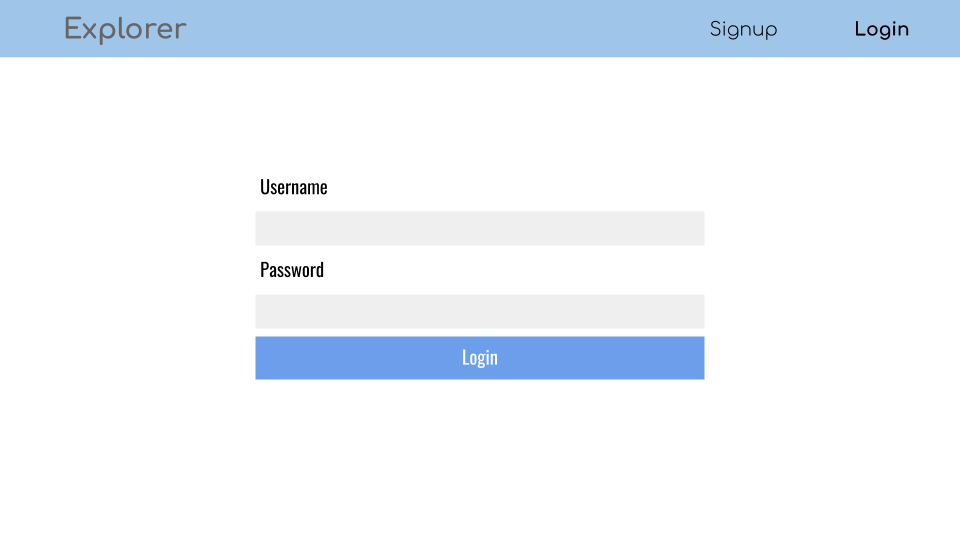
\includegraphics[width = .98\textwidth]{mockups/1.png}}
    \caption{Login/Registration Panel}
    \label{fig:login}
\end{figure}

\begin{figure}[ht]
    \centering
    \fbox{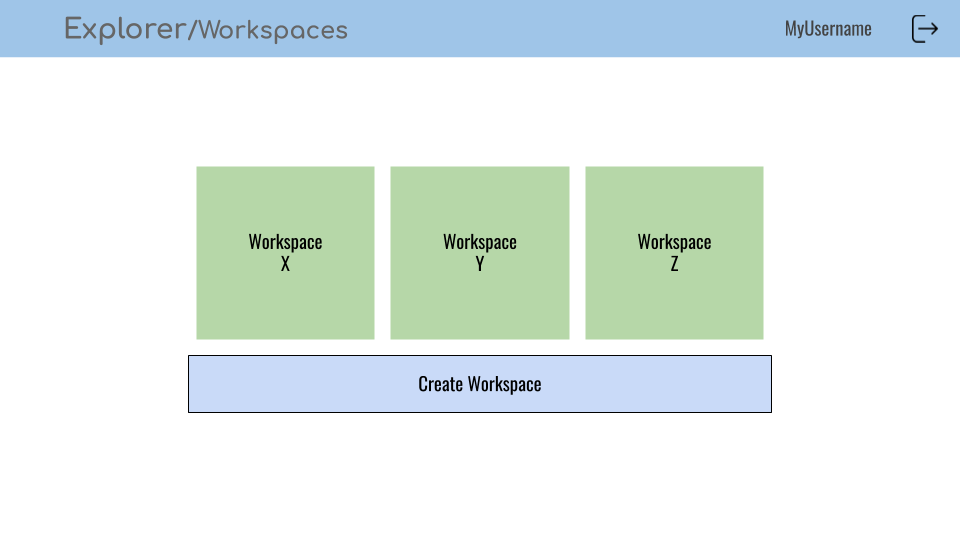
\includegraphics[width = .98\textwidth]{mockups/2.png}}
    \caption{List of current workspaces}
    \label{fig:workspaces-list}
\end{figure}

\begin{figure}[ht]
    \centering
    \fbox{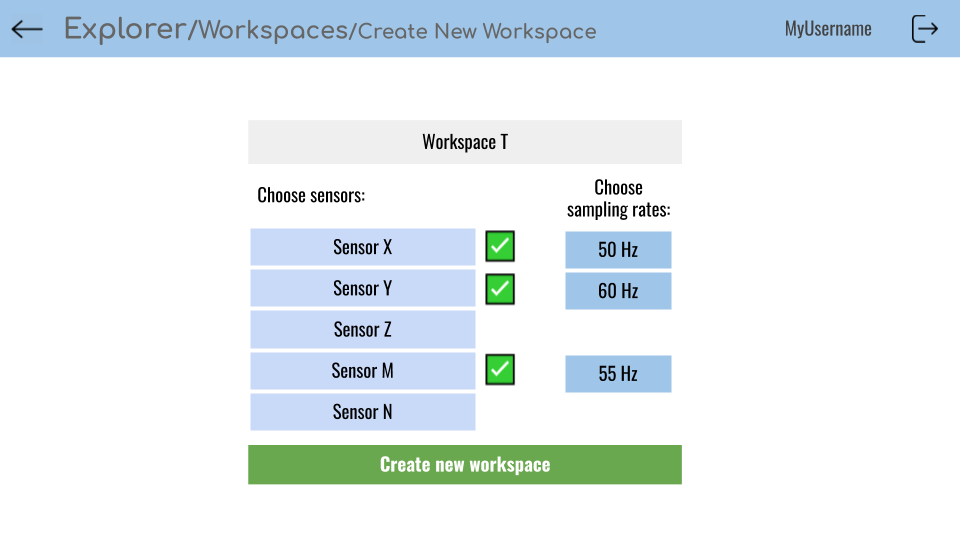
\includegraphics[width = .98\textwidth]{mockups/3.png}}
    \caption{Create a new workspace}
    \label{fig:create-workspace}
\end{figure}

\begin{figure}[ht]
    \centering
    \fbox{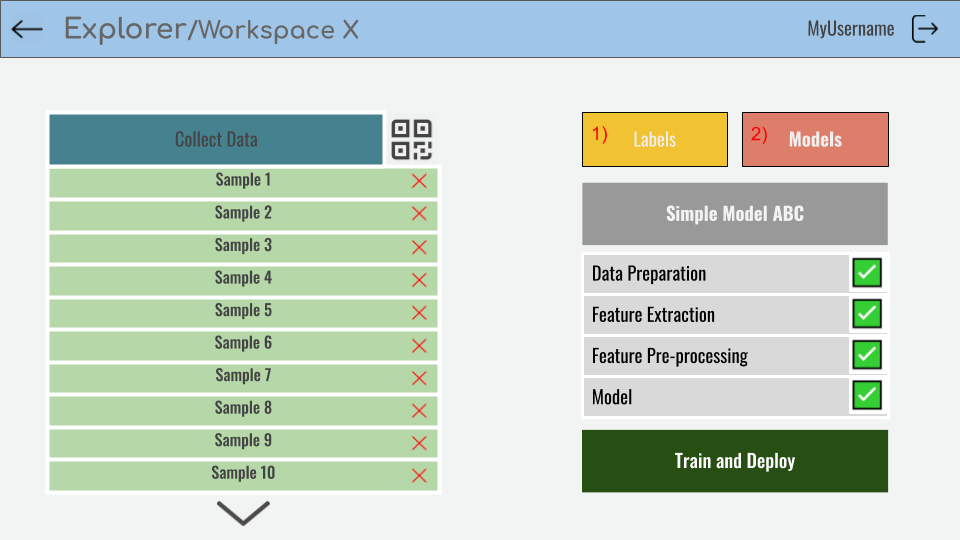
\includegraphics[width = .98\textwidth]{mockups/4.png}}
    \caption{Workspace panel}
    \label{fig:workspace-overview}
\end{figure}

\begin{figure}[ht]
    \centering
    \fbox{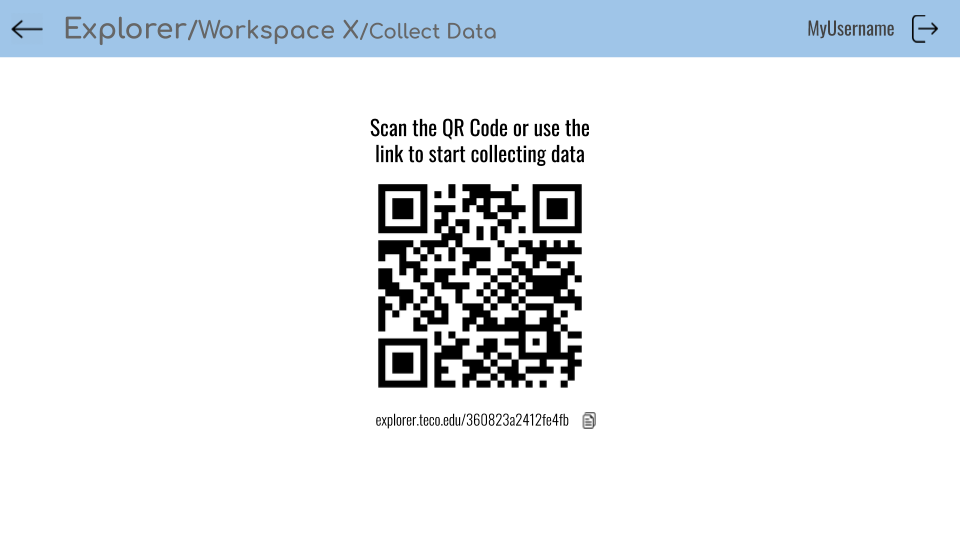
\includegraphics[width = .98\textwidth]{mockups/5.png}}
    \caption{QR Code/Link of workspace to collect data}
    \label{fig:workspace-link}
\end{figure}

\begin{figure}[ht]
    \centering
    \fbox{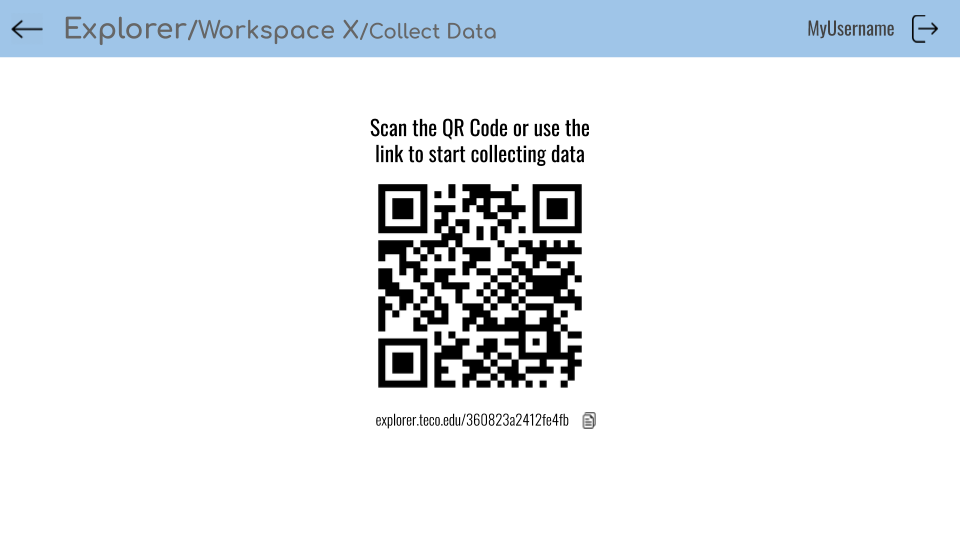
\includegraphics[width = .98\textwidth]{mockups/6.png}}
    \caption{Model training options}
    \label{fig:training-options}
\end{figure}

\begin{figure}[ht]
    \centering
    \fbox{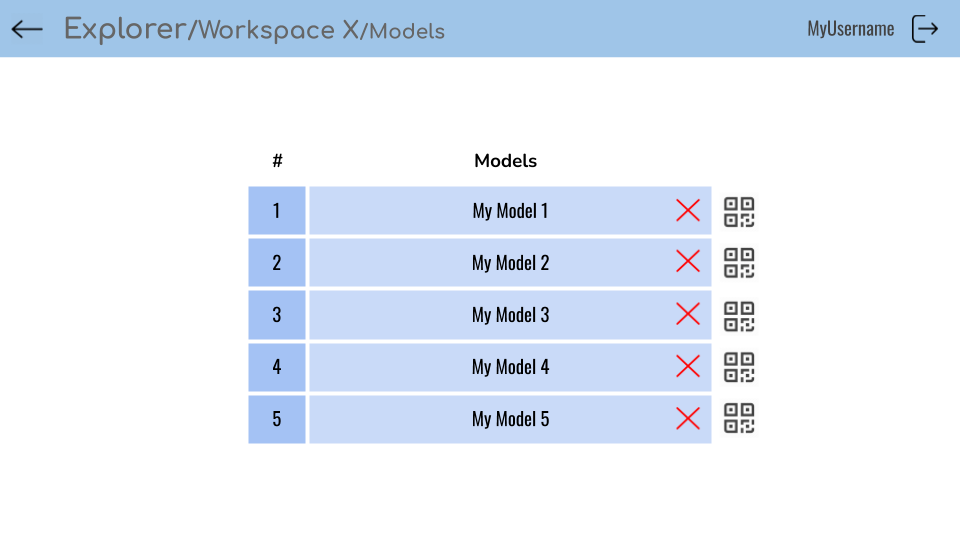
\includegraphics[width = .98\textwidth]{mockups/7.png}}
    \caption{Labels panel}
    \label{fig:labels-panel}
\end{figure}

\begin{figure}[ht]
    \centering
    \fbox{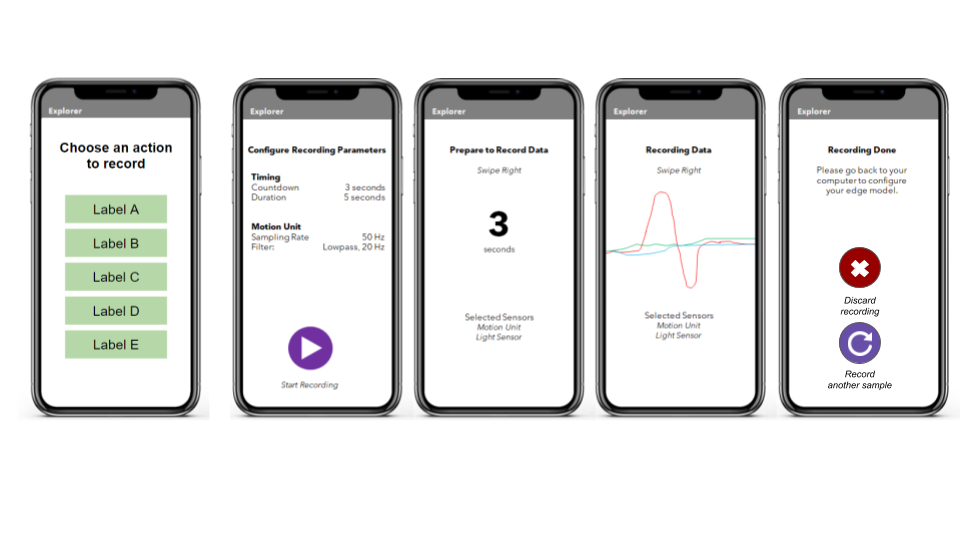
\includegraphics[width = .98\textwidth]{mockups/9.png}}
    \caption{Trained models panel} 
    \label{fig:models-panel} 
\end{figure}

\begin{figure}[ht]
    \centering
    \fbox{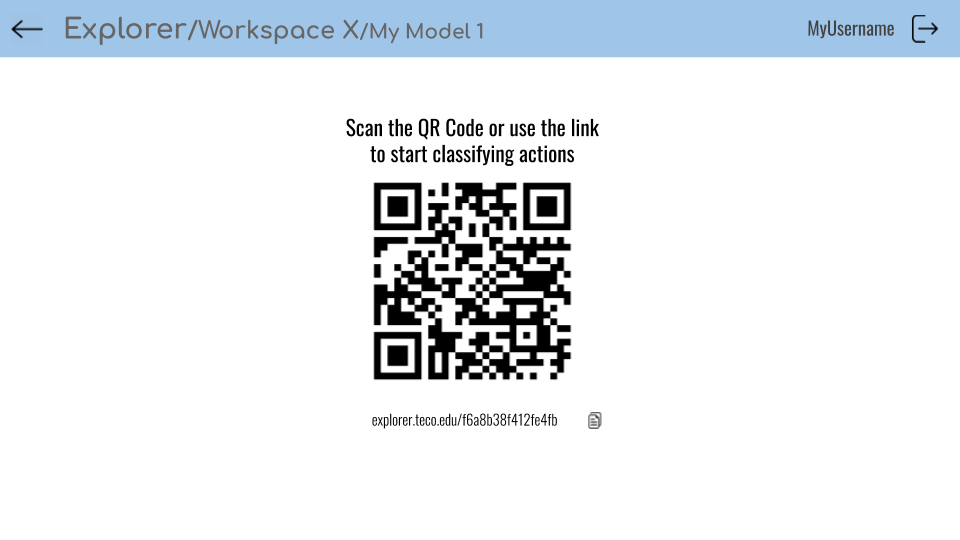
\includegraphics[width = .98\textwidth]{mockups/8.png}}
    \caption{Data sample overview}
    \label{fig:sample-overview}
\end{figure}

\begin{figure}[ht]
    \centering
    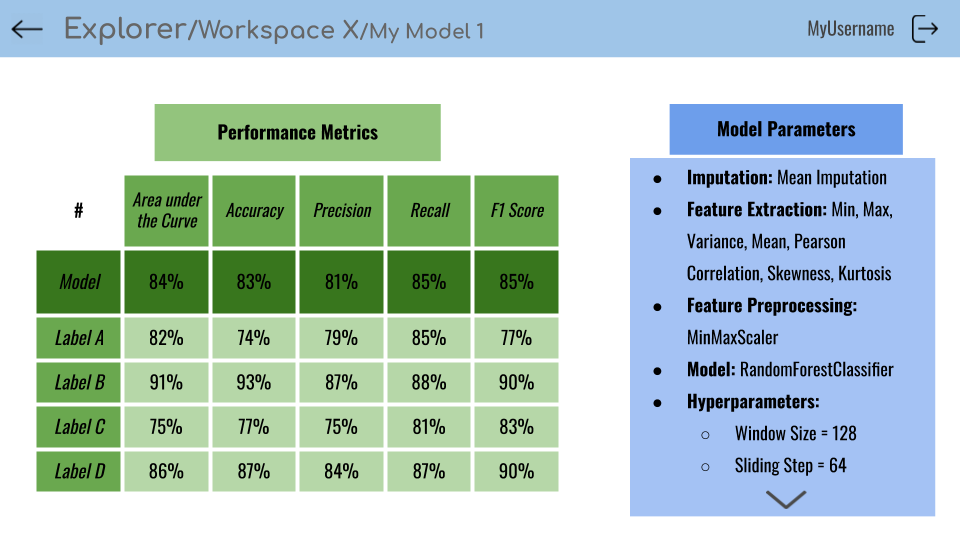
\includegraphics[width = .98\textwidth]{mockups/10.png}
    \caption{Model overview}
    \label{fig:model-overview}
\end{figure}

\begin{figure}[ht]
    \centering
    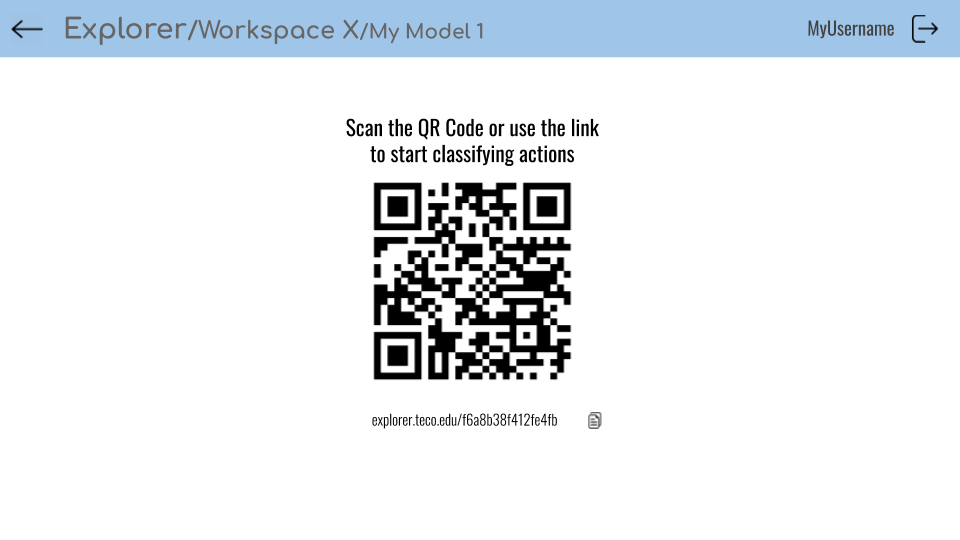
\includegraphics[width = .98\textwidth]{mockups/11.png}
    \caption{QR Code/Link of trained model to classify data}
    \label{fig:model-link}
\end{figure}

\begin{figure}[ht]
    \centering
    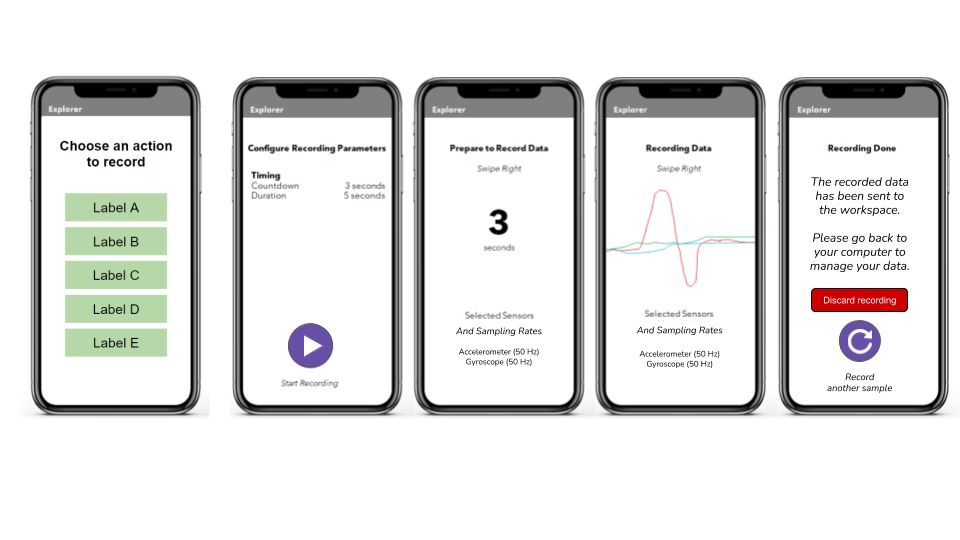
\includegraphics[width = .98\textwidth]{mockups/12.png}
    \caption{Data collection in mobile}
    \label{fig:data-collection}
\end{figure}

\begin{figure}[ht]
    \centering
    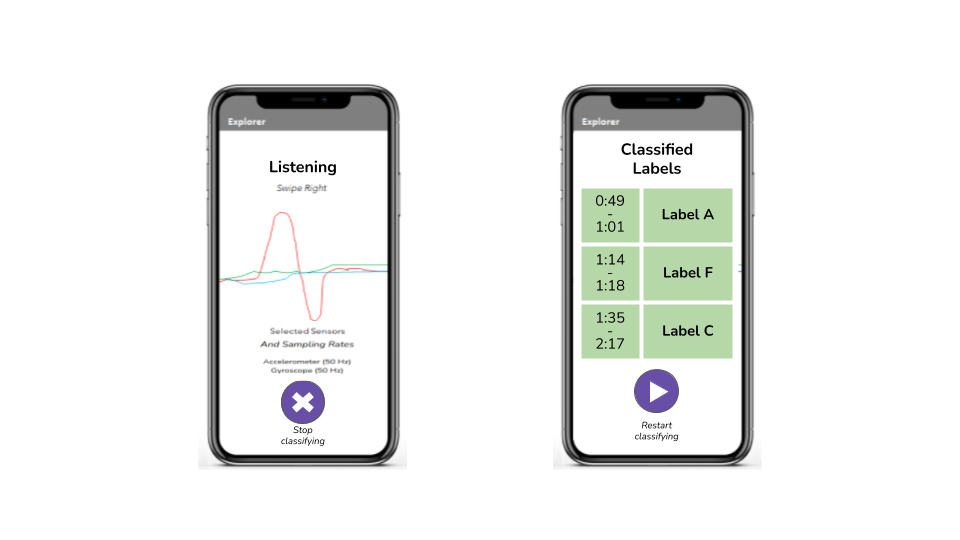
\includegraphics[width = .98\textwidth]{mockups/13.png}
    \caption{Action classification in mobile}
    \label{fig:classification}
\end{figure}